

\documentclass[12pt]{article}
\title{Thellier\_GUI Tutorial}
\date{\today}


\usepackage{amsmath}
\usepackage{graphicx}
\usepackage{url}

\begin{document}
\maketitle


\section{Introduction}

This tutorial describes Thellier\_GUI and its embedded tools. Detailed explanation on the algorithms and methods of calculations can be found in Shaar and Tauxe (2012).  This tutorial refers currently to Mac users only, as the program has not been tested yet on non-mac platform.
 
\section{Opening the GUI and reading data}

\subsection{Starting the GUI}
The GUI can be opened by typing in the Terminal window:\\
pmag\_thellier\_gui.py\\
A "choose project directory" dialog window will appear as soon as the GUI is started (Fig.1) . The Project directory should include a file named "magic\_measurements.txt".  Also, If a file named "rmag\_anistropy.txt" exists, then the program reads the anisotropy data from rmag\_anistropy.txt . Reading and processing the measurements files may take several seconds, depending on the number of the specimens.

\begin{figure}[h!]
	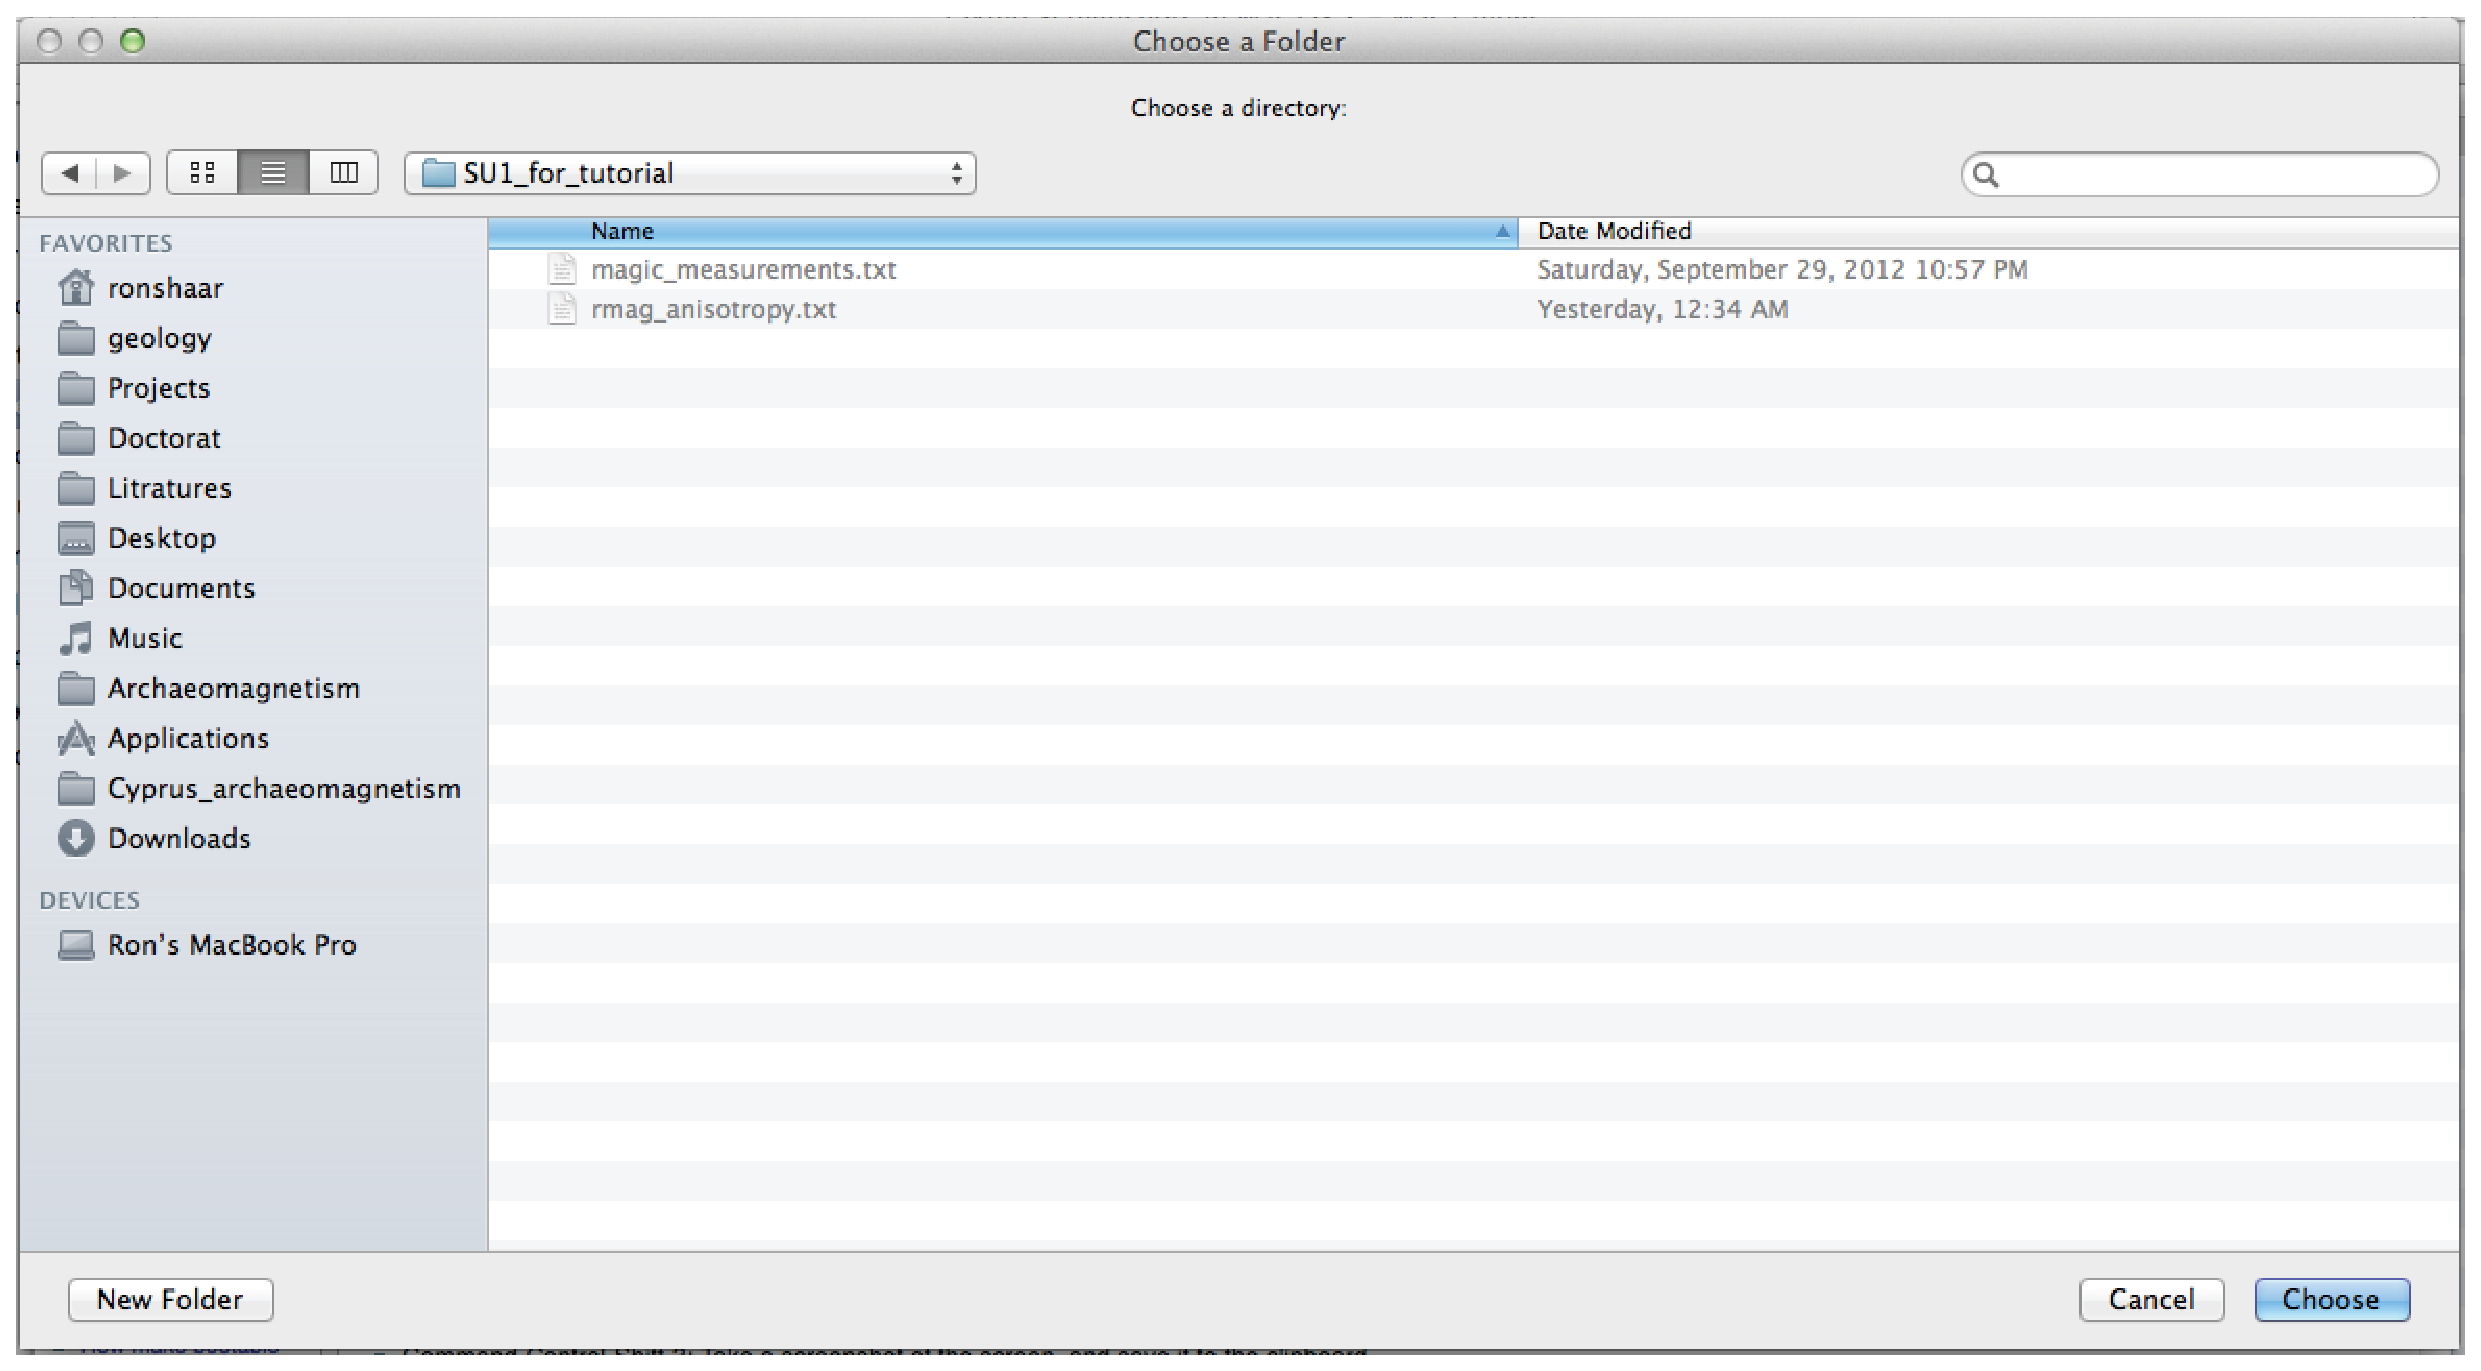
\includegraphics[width=1.0\textwidth]{EPSFiles/Screenshot_choose_directory.eps}
	 \caption{choose project directory dialog}
\end{figure}

\subsection{Reading and compiling measurements data}
When the MagIC project directory is selected, the program  reads all the measurement data, checks it, processes it and sorts it. Messages, warnings and errors regarding the inspection of the data are  stored  in a file named "Thellier\_GUI.log". Each row in Thellier\_GUI.log  starts with "-I-", "-W- WARNING:" or "-E- ERROR:" where the naming convention is -E- is an Error, -W- is a warning, and -I- is Information. The user should inspect Thellier\_GUI.log for Error and Warning.  

\subsubsection{Processing NLT data}
If Non-linear-TRM (NLT) data exist in magic\_measurement.txt then the program tries to process the data using Equations (1)-(3) in Shaar et al. (2010). Several warning may appear. If there are not enough measurements for fitting the the hyperbolic tangent function ($<3$), or if the program cannot fit a hyperbolic function to the data, then the program calculate $max(M/B)/ min(M/B)$ if this value is more than 1.05 but less than 1.1 a warning message will appear. If  this value is greater than 1.1  then an Error message will appear.

\subsubsection{Processing Thellier data}
The program reads "magic\_measurement.txt", and process the measurements for presentation as Arai plot and Zijderveld plot. Error and Warnings may appear if something is wrong with the data. For example: missing zerofield or infield steps, pTRM check is not in place (after infield instead of zerofield), or a non-consecutive order of temperatures.  At the end of the processing the following messages will appear in Thellier\_GUI.log :\\
-I- number of specimens in this project directory:\\
-I- number of samples in this project directory:\\
It is highly recommended to check all the warnings and errors in Thellier\_GUI.log before starting interpreting the data.

\section{Main panel}

\begin{figure}[h!]
	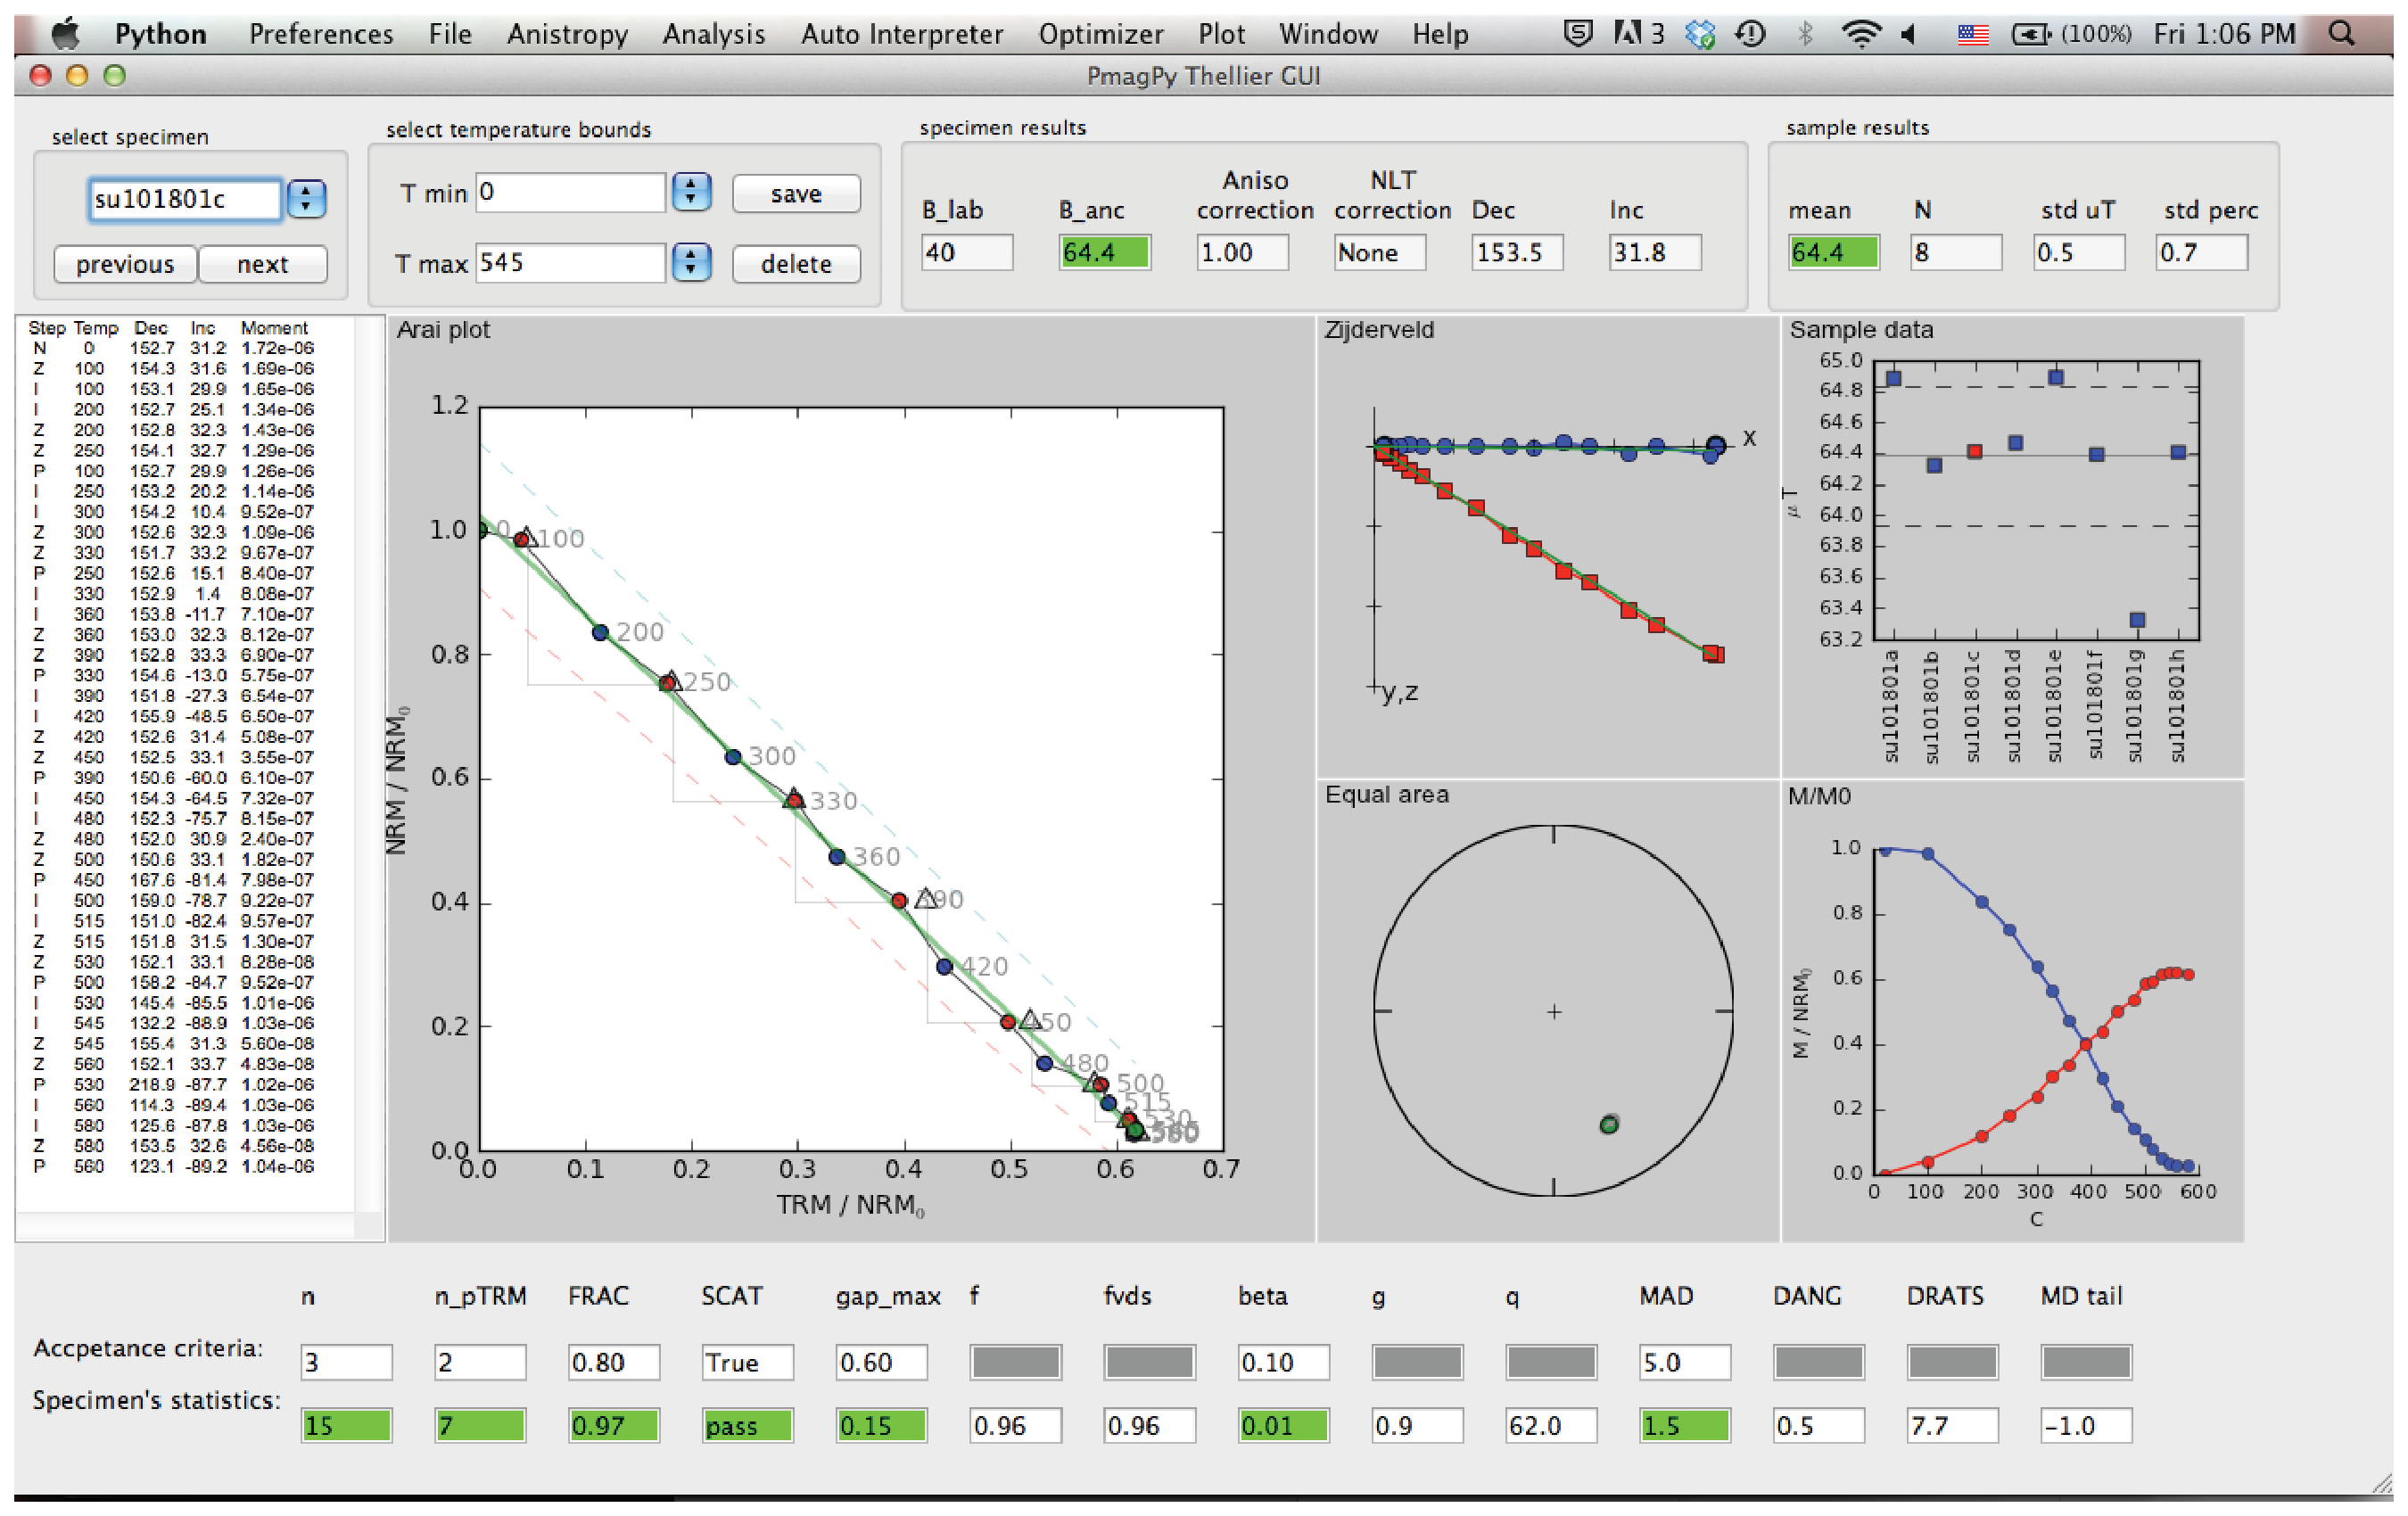
\includegraphics[width=1.0\textwidth]{EPSFiles/Screenshot_main_panel.eps}
	 \caption{Thellier\_GUI main panel}
\end{figure}

Figure 2 shows a snapshot of the main panel. The top field in the  panel includes the following buttons/controls (from left to right):\\
{\bf Specimen:} a list of the specimens in the project folder sorted by name.\\
{\bf previous/next:} buttons to move forward and backward in the specimens list.\\
{\bf T min/T max:} buttons to select temperature bounds.\\
{\bf save/delete:} save or delete current interpretation. This information will be used later to generate a "redo file" \\
\\
{\bf B\_lab:} laboratory field in units of $\mu T$.\\
{\bf B\_anc:} specimen's paleointensity in units of $\mu T$.\\
{\bf Aniso Correction:} anisotropy correction factor.\\
{\bf NLT Correction:} Non-Linear TRM (NLT) correction factor.\\
{\bf Dec/Inc:} Ancient declination/inclination calculated by PCA of the NRM in the selected temperature bounds.\\
\\
The center of the main panel includes the following:\\
{\bf measurements text panel:} Four columns of the measurement data: Step is "N" for NRM, "Z" for zero field step, "I" for infield step, "P" for pTRM check, and "T" for tail check. The temperature of each step is given in C. Also shown  declination, inclination and moment (in units of $Am^2$) \\
{\bf Arai plot:}  Arai plot normalized by $NRM_0$. blue circles are zero field steps, red circles are infield steps, triangles are pTRM checks, blue squares are tail checks. Temperatures are displayed near data points. Temperature bounds and best fit line are marked in green. 'SCAT box' is marked with dashed lines (only if SCAT is True). \\
{\bf Zijderveld plot:}  A Zijdrveld plot of the NRM step.  The x axis is rotated to the direction of the NRM  .blue is the x-y  projection, red is x-z projection.\\
{\bf Equal area plot:}  An equal area projections  of the NRM steps. solid circles are positive inclination. open circles are negative inclinations.\\
{\bf Moment-temperature plot:}  NRMs are in blue, pTRMs are in red.\\
{\bf sample data:}  If at least two specimens have a saved interpretation, then their values are displayed on this plot. The mean $\pm$ standard deviation of the mean are marked as  horizontal lines. \\
\\
The bottom of the main panel include paleointensity statistics. The first line is the threshold values (empty if N/A). The second line is the specimen's statistics. For details see Appendix A1 in Shaar and Tauxe (2012).

\section{Menu bar}
\subsection{File menu bar}
{\bf Open MagIC project directory:} Open a dialog window for choosing a new project directory.\\
{\bf Open MagIC measurement file:} Open a dialog window for choosing a new magic measurement file.\\
{\bf Save plot:} save the current display of the Arai plot, Zijderveld plot, Equal area projection, and M plot. The default options for saving the figures are pdf,svg, and eps. To save in another format the appropriate suffix should be added to the file name (python supported formats are emf, eps, pdf, png, ps, raw, rgba, svg, svgz)\\

\subsection{Analysis menu bar}
{\bf Acceptance criteria   $\rightarrow $  Set Accpetance criteria to default: } Change acceptance criteria to default values.\\
{\bf Acceptance criteria   $\rightarrow $  Change acceptance criteria: } Import a dialog box for setting acceptance criteria and sample's calculation methods . For details on each definition in the Acceptance criteria dialog box see Appendix A1 in Shaar and Tauxe (2012).\\
{\bf Acceptance criteria   $\rightarrow $  Import criteria filet: } Open criteria from an existing pmag\_criteria.txt file. \\
{\bf Import previous interpretation ('redo file'):} Open a "redo file" that includes previous interpretations. The "redo file" is tab-delimited txt file with three fields. the first field is specimen name, the second is minimum temperature bound (in Kelvin, whereas NRM is 273), and the third field is the maximum temperature bound.\\
{\bf Save current interpretation:} Save the current interpretation and create the following files in the project directory:\\
thellier\_GUI.redo: A redo file that includes the temperature bounds of all the saved interpretation.\\
thellier\_GUI.specimens.txt: A text file that includes the interpretation of all the saved specimens, and the values of their paleointensity statistics. The first three lines are the acceptance criteria defined at the time the data was saved.  The rest of the file is a list of the specimen's data sorted by specimen's name.  The last columns is Pass/Fail - if the specimen fail the criteria, the list of the failed parameters is given. This file is useful for preparing the final table for publication.\\
thellier\_GUI.samples.txt: A text file that includes the statistics of the samples. All the samples are included in this list regardless the sample's acceptance criteria. This file is useful for preparing the final table for publication.\\
{\bf Clear all current interpretation:}  Clear all the saved interpretations.\\

\begin{figure}[h!]
	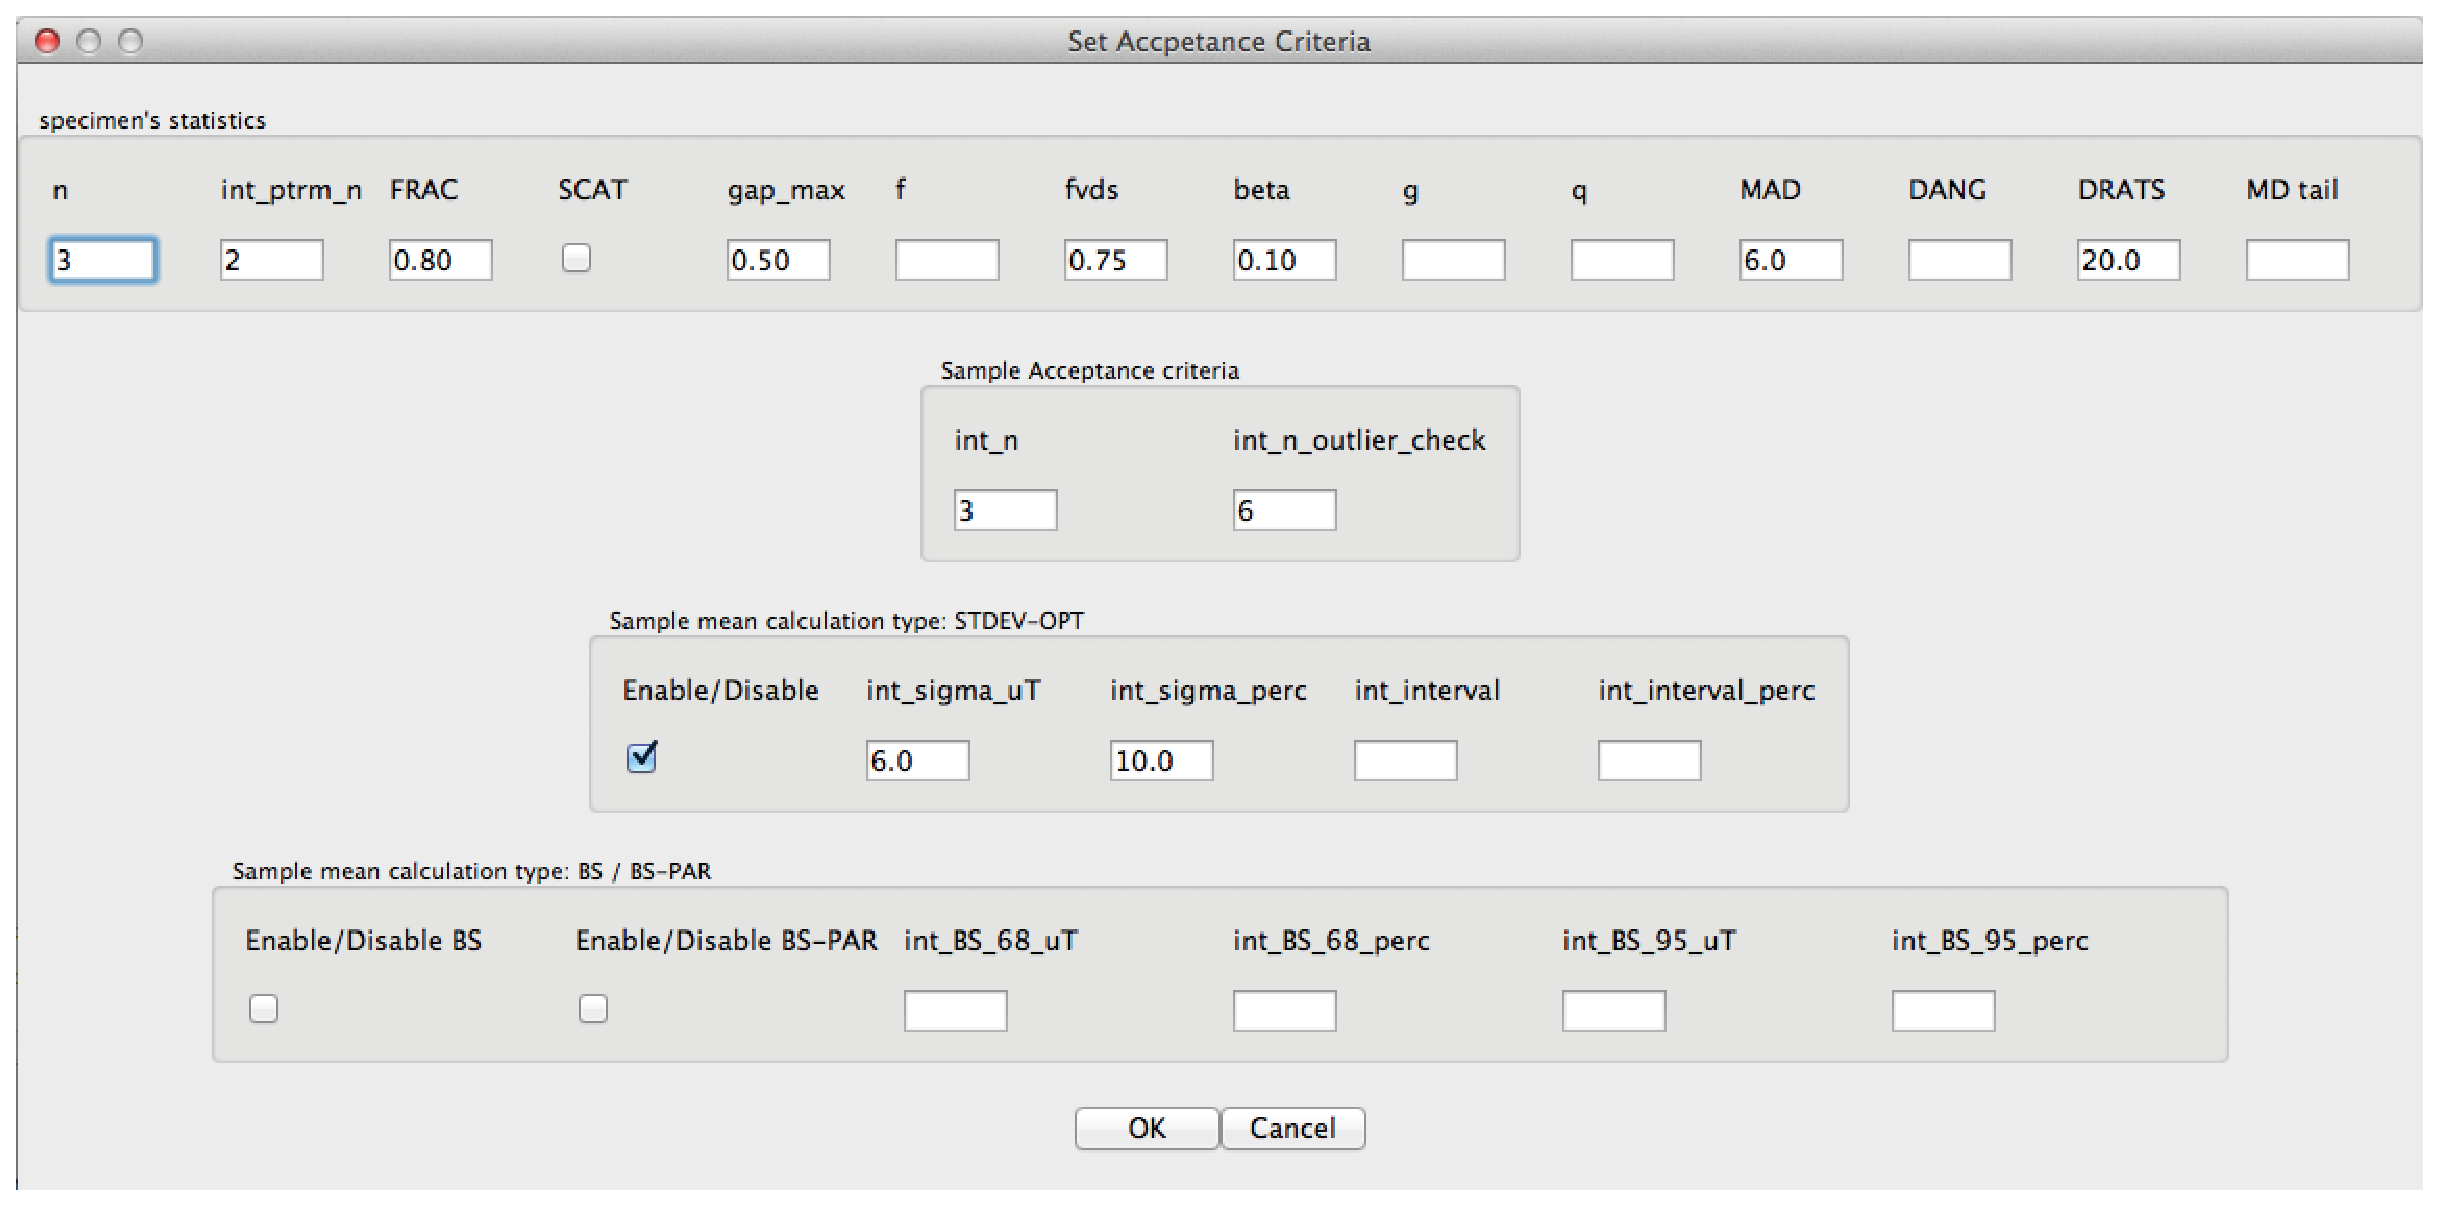
\includegraphics[width=1.0\textwidth]{EPSFiles/Screenshot_criteria_dialog.eps}
	 \caption{Setting  acceptance criteria and sample's mean calculation method. For explanation on each parameter see Appendix in Shaar and Tauxe (2012) }
\end{figure}


\subsection{Auto Interpreter menu bar}
{\bf Run Thellier auto interpreter:} Run  {\it Thellier\_auto\_interpreter} using the current acceptance criteria and sample's mean calculation method.\\
\\
 \underline{ \textbf{ Thellier\_auto\_interpreter output files } }\\
{\it Thellier\_auto\_interpreter} produces the following output files in a directory named "thellier\_interpreter":\\
{\bf thellier\_interpreter.log}\\
A log file. Each line in the log file starts with-I- (Information), -W- (Warning), or -E- (Error). The first massages/errors/warnings include reading the measurement data, sorting, and processing the data (similar to Thellier\_GUI.log). Then, each trial is given, for example:\\
-I- specimen su100301a (200-500) FAIL on: specimen\_frac= 0.799844, \\ 
-I- specimen su100301a (200-515) PASS\\
The end of the log files include the samples mean calculation.\\
{\bf thellier\_interpreter\_specimens\_bounds.txt:}\\
A summary file that lists the minimum and the maximum of the 'acceptable interpretation' (for specimens  that have at least one 'acceptable' interpretation). The first four lines in the file are the acceptance criteria used. The next line is a header, and then the data for all the specimens: sample name, specimen name, anisotropy correction factor, anisotropy correction type, NLT correction factor, lab field (uT), minimum 'acceptable' interpretation, maximum 'acceptable' interpretation, and Warning. This file is useful for inspecting the behavior of the dataset in general. \\
{\bf thellier\_interpreter\_all.txt}\\
A file that contains all the accepted interpretations (temperature bounds, pale intensity values, and statistics) for all the specimens. There may be more than one 'acceptable' interpretation for each specimen.\\
{\bf thellier\_interpreter\_STDEV-OPT\_samples.txt}\\
A summary file with all the samples that passed the criteria. The first four lines are the acceptance criteria used in the interpretation. Then, the following information is given: sample name, number of specimens used in the calculation, the paleointensity in units of $\mu T$,  standard deviation of the sample mean in units of $\mu T$, standard deviation divided by the mean in units of \%, Interval of accepted sample means in units of $\mu T$,  Interval of accepted sample means divided by the sample's mean in units of \%, Warning.This information is useful for generating a table for a publication. \\
{\bf thellier\_interpreter\_STDEV-OPT\_specimens.txt}\\
A list of the specimen's interpretations that were chosen by STDEV-OPT algorithm to produce the sample's mean, and the paleointensity statistics. This information is useful for generating a table for a publication.\\
{\bf thellier\_interpreter\_STDEV-OPT\_redo}\\
A "redo" file (see section 4.2) This is a tab-delimted text file with three fields: the first field is specimen name, the next is minimum temperature bound (in Kelvin, whereas NRM is 273), and the third field is the maximum temperature bound. \\
{\bf thellier\_interpreter\_BS\_samples.txt}\\
A summary file with all the samples that passed the criteria in the bootstrap method (only if BS method is used for sample calculation).\\
{\bf thellier\_interpreter\_BS-PAR\_samples.txt}\\
A summary file with all the samples that passed the criteria in the parametric bootstrap method only if (BS method is used for sample calculation).\\
\\
{\bf Open auto interpreter output file:}  Open output files of the Thellier\_interpreter and present it on a table. The first lines with the acceptance criteria are not displayed.\\

\subsection{Thellier\_optimizer\_2d}
Thellier\_optimizer\_2d is a built-in self test for the consistency of the data among 'test groups' (see Shaar and Tauxe, 2012 for details).\\
The Thellier\_optimizer\_2D requires definition of 'test groups',  'test functions', and 'fixed\_criteria'.\\
 \underline{ \textbf{ Test groups }}\\
Test groups include samples that are expected to give  similar paleointensity results. The test groups are defines in an "er\_sample" file (tab delimited). The first line in this file is:\\
tab 	er\_samples.\\
The next line is the header, which must include at least the following:\\
er\_sample\_name	 er\_group\_name.\\
(Another header "comments" is recommended).\\
The rest of the lines are the sample names and the group names. (see the example below). \\
 \underline{ \textbf{ fixed\_criteria }}\\
fixed\_criteria are the list of threshold values  for paleointensity statistics, not including frac and $\beta$. When selecting Optimizer $\rightarrow$ Run Thelllier Optimizer, a criteria dialog window (fig. 3) is opened in order to set the "fixed\_criteria".\\ The fixed criteria are saved in a file named "pmag\_fixed\_criteria.txt" in a folder named "optimizer".\\
 \underline{ \textbf{ Thellier\_optimizer\_2d Dialog window: Test functions and run definitions }}\\
 Fig. 4 show the  Thellier\_optimizer\_2d dialog window. \\
The upper control buttons select the range of $\beta$ and  FRAC.\\
test functions are entered in the main text panel.\\
The button "Check function syntax" is used to check if the functions can be compiled. If the functions are valid the text window will show "PASS", otherwise it shows "FAIL". \\
The button "choose optimizer group file" opens a file dialog for choosing the er\_sample file with the 'test groups'.\\
The button "Run optimizer" start the optimizer.\\
\\
 \underline{ \textbf{  Thellier\_optimizer\_2d output files }}\\
All Thellier\_optimizer\_2d output files are saved in a folder named optimizer in the project directory.\\
{\bf optimizer\_functions.txt}\\
 This file saves the test functions as entered in the Thellier\_optimizer\_2d  dialog window.\\
{\bf pmag\_fixed\_criteria.txt}\\
 This file saves the fixed\_criteria used by Thellier\_optimizer\_2d.\\
{\bf thellier\_optimizer.log}\\
Log file. \\
{\bf thellier\_optimizer\_interpretation\_log.txt.gz}\\
This log file includes information on all the iteration over all the specimens using all the sets of criteria. Since this is a big file, it is saved in a gzip compressed format.\\
 {\bf optimzer\_results.txt}\\
A summary files of the optimizer results. Each line includes the following: FRAC, beta, test-site name, name of samples that passes separated by :, sample's paleointensities in microT, arranged in the same order as samples' names, test-site mean, test site standard deviation, test site standard deviation divided by its mean.\\
\\
Color maps of the test functions are saved in pdf format (under a folder named "pdf") and in svg format (under a folder named 'svg').

\begin{figure}[h!]
	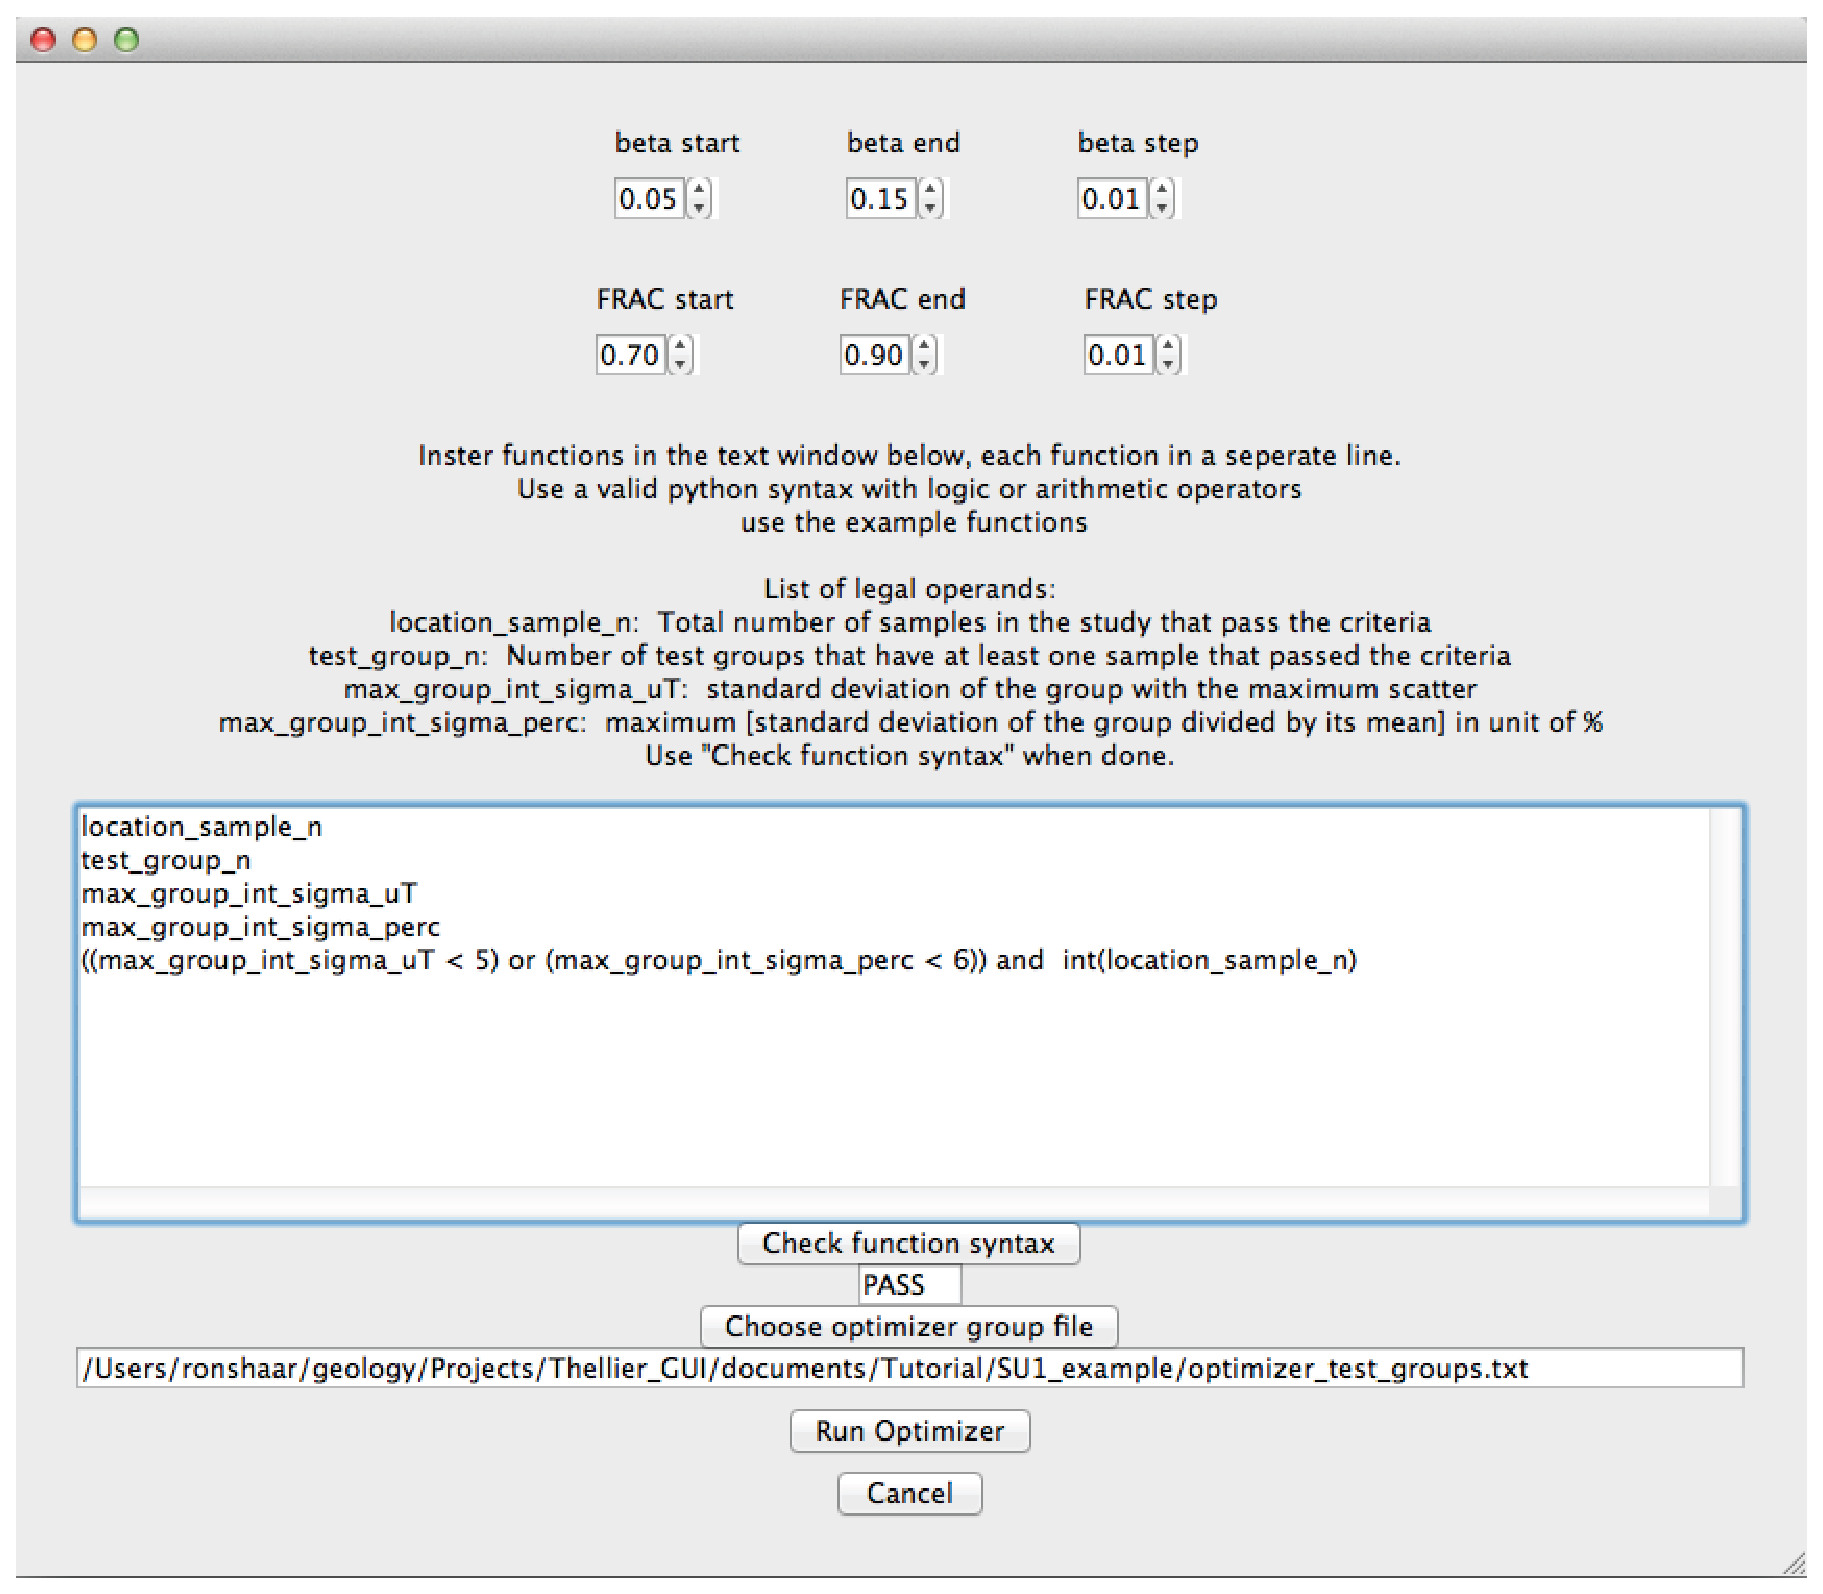
\includegraphics[width=1.0\textwidth]{EPSFiles/Screenshot_optimizer_dialog.eps}
	 \caption{Thellier\_optimizer\_2D dialog window}
\end{figure}


\section{ Tutorial by example}
\subsection{Getting started}

\begin{itemize}
\item If PmagPy is not installed yet on your computer follow the instructions in MagIC cookbook chapters 1 and 5:\\ \url{http://earthref.org/PmagPy/cookbook/}).
\item If PmagPy is installed, download the latest version of PmagPy from\\ \url{https://github.com/ltauxe/PmagPy}.
\item Download  example data files for PmagPy from\\  \url{http://earthref.org/PmagPy/Datafiles_2.0.zip}\\ 
 There are two folder located under the folder "thellier\_gui": SU1\_example and Tauxe\_2006\_example.
\end{itemize}
\subsection{Case study 1: SU1\_example}
Open a new Terminal window. Type "thellier\_gui.py" and press enter. A choose directory dialog window will appear. Select the SU\_1 project directory. click on the "choose" button.
\subsubsection{Manual interpretation}
Manual interpretation is the conventional approach of selecting temperature bounds for each specimen. Here, as example, we will interpret one sample, su100601,  manually.
\begin{itemize}
\item Set acceptance criteria: From the menu-bar choose  Analysis $\rightarrow$ Acceptance criteria $\rightarrow$ Change acceptance criteria. A criteria dialog box will appear.
\item In the first line (specimen's statistics) set the following values: n=3, int\_ptrm\_n=2, SCAT=false (unchecked), gap\_max=0.5, f\_vds=0.75, beta=0.1, MAD=6, DRATS=20. delete the values in the other boxes (empty boxes). \\
In the second line (Sample's acceptance criteria) set the following values: int\_n=3. delete the value in the other boxes.\\
In the third row (Sample mean calculation method: STDEV-OPT) check the Enable/Disable box, and set the following values: int\_sigma=6, int\_sigma\_perc=10. Delete values in the other boxes. Figure 3 shows how it should look. click on the OK button. A message dialog will appear telling you the criteria that you chose are saved in a file name pmag\_criteria.txt. The next time you will open the GUI in this project directory, these criteria will automatically be chosen. Click OK on the message box.
\item Manual interpretation of sample su100601: choose specimens su100601a from the specimen list. choose temperature bounds from the Tmin/Tmax windows: 200 and 580. B\_anc shows 61.7 in green, which means that this interpretation passes the specimen's acceptance criteria. Now, change Tmax to 530.  B\_anc window change color to red, and also the fvds window (the row on the bottom of the GUI). This is an indication that the interpretation did not meet the criterion for fvds. Change  Tmax to 580 (as before) and press "save" button. The interpretation in saved. 
\item Click on the next button to choose the next specimen (su100601b). Before analyzing this specimen, press on the "previous" button, so you can see that your previous interpretation was saved. click on "next" to return again to specimen su100601b. Find  temperature bounds that pass the criteria (for example 200,580). Make sure that all colors are green, and click on the "save" button. Go over all the other specimens in the sample (su10060a to su100601g). you will find that three specimens can pass: a,c, and g. Look at the Sample data figure (top right) it shows the saved interpretation for all the specimens in the sample, and the mean $\pm$  standard deviation of the mean. 
\item To save all your interpretation into files, choose from the menubar Analysis $\rightarrow$ Save current interpretation. Three files will be generated in the project directory:\\
1. thellier\_GUI.redo (the temperature bounds for each specimen):\\
su100601a 473 853\\
su100601c 473 853\\
su100601g 473 853\\
( notice that the temperature bounds are in Kelvin)\\
2. thellier\_GUI.specimens.txt (the paleointensity statistics for each specimen - according to the headers. It is easy to view the content of this file using Exel):\\
su100601a	su100601	61.7	200	580	40.0	1.07	1.01	15	8	0.77	0.87	0.89	0.14	0.02	N/A	0.63	N/A	5.11	4.14	PASS\\
su100601c	su100601	54.4	200	580	40.0	0.94	N/A	15	8	0.60	0.78	0.79	0.23	0.01	N/A	5.19	N/A	2.51	1.33	PASS\\
su100601g	su100601	58.4	200	580	40.0	1.00	1.01	15	8	0.70	0.83	0.85	0.19	0.02	N/A	2.80	N/A	3.12	1.96	PASS\\
3. thellier\_GUI.samples.txt (the paleointensity statistics of the samples):\\
er\_sample\_name	sample\_int\_n	sample\_int\_uT	sample\_int\_sigma\_uT	sample\_int\_sigma\_perc\\
su100601	3	58.2	3.0	5.1\\
\item You can save the Arai plot (or any other plots) from the File menu. Choose  file  $\rightarrow$ Save Plot $\rightarrow$ Save Arai plot. A file dialog window will appear. You can change the format of the figure in the bottom tab (pdf, svg, or png), but you can also save as other format by adding the appropriate suffix to the file name.
\item close the GUI: File  $\rightarrow$ Quit.
\item Re-open the GUI like before ( by writing the command  "thellier\_gui.py"  in the terminal box) and choose the same working directory (SU1\_example). Notice, that the criteria that you set before are automatically used. To import your previous interpretations and continue working on this dataset choose from the menu bar Analysis $\rightarrow$ import previous interpretation. Choose thellier\_GUI.redo and click on the 'open' button.
\end{itemize}
\subsubsection{Automatic interpretation - \it{thellier\_auto\_interpreter}}
Instead of trying to find manually the most appropriate temperature bounds, the  thellier\_auto\_interpreter allows a fast and consistent way to choose the temperature bounds for the specimens. For details see Shaar and Tauxe (2012). 
\begin{itemize}
\item We will use the same acceptance criteria, which were set on the previous section. If you are not sure about that, go back to the second bullet in section 5.1. 
\item Choose from the menu bar Auto interpreter $\rightarrow$ Run Thellier auto interpreter. The interpreter will run approximately 30 seconds. When its done, a message window will appear saying that the interpreter finished successfully (if not, check for errors in the terminal window, or in a file name "thellier\_interpreter.log"  located in a folder name "thellier\_interpreter". If the issue cannot be resolved send e-mail with the description of the problem to rshaar@ucsd.edu). Click OK in the message window.
\item The automatic interpretations are automatically saved, and we can review them on the Arai plots.  Lets look, for example, on the sample we interpreted  manually: su100601. Choose specimen su100601a from the specimens list. In a first look the choice seems strange because the automatic interpretation chose temperature bounds 0 and 580. A choice between 200 and 580 may seem more reasonable as it provides an nearly straight line. The sample data figure explains this issue. The thellier\_auto\_interpreter chooses the interpretations that minimize the standard deviation of the sample's mean. Six specimens from this sample passed the criteria, and the value of su100601a is much higher than the remaining five. So, the thellier\_auto\_interpreter chose the 'acceptable' interpretation with the shallowest  slope. Go over the other specimens in the sample, and review the automatic interpretation. If you want, you can change the automatic interpretation, and save your own "manual" interpretation by choosing Analysis $\rightarrow$ Save current interpretation. Notice, that the output of thellier\_auto\_interpreter is sensitive to the choice of the acceptance criteria, and different criteria may lead to significantly different final results. 
\end{itemize}
\subsubsection{Choosing the optimal criteria - \it{thellier\_optimizer\_2D}}
Shaar and Tauxe (2012) discuss a method to choose the optimal specimen's acceptance criteria. Here, we follow the example given in this paper. Shaar and Tauxe (2012) suggested using  seven statistics for specimen's acceptance criteria. The choice of four of which is trivial, and the remaining three are MAD, FRAC and $\beta$. The thellier\_optimizer\_2D helps finding the optimal values for FRAC and $\beta$.  The thellier\_optimizer\_2D  required three types of inputs: 'fixed\_criteria", "test\_groups", and "test\_samples", as decried below:  
\begin{itemize}
\item The test groups are defined in an "er\_sample" file. An example for this file is given in working folder SU-1 named  "optimizer\_test\_groups.txt". Open this file in Excel to understand its syntax. The first line is a general header. The rest of the file include sample name, group name, and comments. 
\item To run the optimizer choose from the menu bar Optimizer $\rightarrow$ Run Thellier optimizer. click OK in the  message dialog. The first step is setting the 'fixed\_criteria". We choose for the specimen's criteria: n=3, int\_ptrm\_n=2,SCAT=checked, gap\_max=0.6, MAD=5.0. We choose for the sample's criteria:int\_n=3, int\_n\_outlier\_check=6, EnableSTDEV-OPT, int\_sigme\_uT=5, int\_sigma\_perc=6. The rest of the boxes should be empty. click OK. click OK on the message window that will appear.
\item The thellier\_optimizer\_2D dialog window will appear. The first two rows of controls for choosing the range for $\beta$ and FRAC. choose beta from 0.05 to 0.15 in steps of 0.1 and FRAC from 0.7 to 0.9 in step of 0.02. \\
Inert the following functions to the text panel:\\
study\_sample\_n\\
max\_group\_int\_sigma\_uT\\
((max\_group\_int\_sigma\_uT $<$= 5) or (max\_group\_int\_sigma\_perc $<$= 6)) and  int(study\_sample\_n) \\
click on the "Check function syntax" button. If there are no typos, then the text box below the button should be PASS.\\
click on the "Choose optimizer group file" button. A file dialog window will appear. choose the file "optimizer\_test\_groups.txt". Click the button "Run Optimizer" to start. The runtime using these parameter is about 8 minutes. `
\item All the output files of the optimizer are saved in a folder named "optimizer" (see section 4.4). Compare the figures in the 'pdf' folder with Figure 7 in Shaar and Tauxe (2012).  
\item The figure in optimization\_function\_2.pdf suggest using $\beta \leq$0.10 and FRAC  $ \geq $0.79. Set these values as acceptance criteria, and run thellier\_auto\_interpreter.  

\end{itemize}
\subsection{Case study 2: DSDP/ODP submarine basaltic glass collections}
This case study follows the second case study  in Shaar and Tauxe (2012). 
\subsubsection{thellier\_auto\_interpreter}
\begin{itemize}
\item Open a new Terminal window. Type "thellier\_gui.py" and press enter. A choose directory dialog window will appear. Select the project directory: Tauxe\_2006\_example. click on the "choose" button.
\item  Set the acceptance criteria: From the menu-bar choose  Analysis $\rightarrow$ Acceptance criteria $\rightarrow$ Change acceptance criteria. A criteria dialog box will appear. In the first line (specimen's statistics) set the following values: n=2, int\_ptrm\_n=2, SCAT=false (unchecked), gap\_max=0.5, f\_vds=0.2, beta=0.1, MAD=15, DRATS=30, DANG=15. delete the values in the other boxes (empty boxes). For the sample's acceptance criteria choose: int\_n=2,  Enable STDEV-OPT, int\_sigme\_uT=5, int\_sigma\_perc=15. Click OK.
\item Choose from the menu bar Auto interpreter $\rightarrow$ Run Thellier auto interpreter. The automatic interpretation takes about 1.5 minutes.. A message dialog will appear when the program is done. With the "previous" and "next" buttons review the automatic interpretation. 
\end{itemize}

\subsubsection{Choosing the optimal criteria - \it{thellier\_optimizer\_2D}}
\begin{itemize}
\item To run the optimizer choose from the menu bar Optimizer $\rightarrow$ Run Thellier optimizer. click OK in the  message dialog. The first step is setting the 'fixed\_criteria". We choose for the specimen's criteria: n=3, int\_ptrm\_n=2,SCAT=checked, gap\_max=0.6, MAD=10.0. We choose for the sample's criteria:int\_n=2,, EnableSTDEV-OPT, int\_sigme\_uT=5, int\_sigma\_perc=15. The rest of the boxes should be empty. click OK. click OK on the message window that will appear.
\item The thellier\_optimizer\_2D dialog window will appear. The first two rows of controls for choosing the range for $\beta$ and FRAC. choose beta from 0.05 to 0.27 in steps of 0.02 and FRAC from 0.30 to 0.86 in step of 0.02. \\
Inert the following functions to the text panel:\\
location\_sample\_n\\
max\_group\_int\_sigma\_uT\\
((max\_group\_int\_sigma\_uT $<$= 5) or (max\_group\_int\_sigma\_perc $<$= 15)) and  int(location\_sample\_n) \\
click on the "Check function syntax" button. If there are no typos, then the text box below the button should be PASS.\\
click on the "Choose optimizer group file" button. A file dialog window will appear. choose the file "er\_test\_groups.txt". Click the button "Run Optimizer" to start. The runtime using these parameter is about 20 minutes. Compare the results with Fig 10 in Shaar and Tauxe (2012)


\end{itemize}

%to su100901h, and choose temperature bounds (using Tmin Tmax buttons that) yield green colors in all windows. after finding for each specimen the best interpretation according to your judgment press "save" to save the interpretation. Make sure that you find successful interpretation for at least two specimens.  You will get something similar to Fig. 6. Notice that your interpretation can be views on the "Sample data" plot (top right go the panel). Save your interpretation by choosing from the menu-bar Analysis $\rightarrow$ Save current interpretation. The program will create a file called "thellir\_GUI.redo" in the project directory.\\
%
%
%
%1.2. In the terminal window change directory to SU1\_example, and type "thellier\_gui.py". \\ \\
%1.3. A "close MagIC project directory" dialog will appear. choose folder SU1\_example and press OK. \\ \\
%1.4. Using "previous" and "next" button move across the specimens, or choose specimens from the "specimen" window. \\ \\
%1.5. Manual interpretation / Set acceptance criteria: From the menu-bar choose  Analysis $\rightarrow$ Acceptance criteria $\rightarrow$ Change acceptance criteria. A criteria dialog box will appear.\\ \\
%In the first line (specimen's statistics) set the following values: n=2, int\_ptrm\_n=2, SCAT=false (unchecked), gap\_max=0.5, f\_vds=0.8, beta=0.1, MAD=6, DRATS=20. delete the values in the other boxes (empty boxes). \\ \\
%In the second line (Sample's acceptance criteria) set the following values: int\_n=3. deleted the value in the other box.\\
%In the third row (Sample mean calculation method: STDEV-OPT) check the Enable/Disable box, and set the following values: int\_sigma\_n=6, int\_sigma\_perc=10. Delete values in the other boxes. Figure 5 shows how it should look.\\ \\
%1.6 Manual interpretation sample su100901: choose specimens su100901a to su100901h, and choose temperature bounds (using Tmin Tmax buttons that) yield green colors in all windows. after finding for each specimen the best interpretation according to your judgment press "save" to save the interpretation. Make sure that you find successful interpretation for at least two specimens.  You will get something similar to Fig. 6. Notice that your interpretation can be views on the "Sample data" plot (top right go the panel). Save your interpretation by choosing from the menu-bar Analysis $\rightarrow$ Save current interpretation. The program will create a file called "thellir\_GUI.redo" in the project directory.\\
%1.7 
%
%Exit the GUI (File $\rightarrow$ Quit). and reopen the GUi using 
%
%
%\begin{figure}[h!]
%	\includegraphics[width=1.0\textwidth]{EPSFilesScreenshot_example_1}
%	 \caption{Acceptance criteria for Example 1.5}
%\end{figure}
%
%\begin{figure}[h!]
%	\includegraphics[width=1.0\textwidth]{EPSFilesScreenshot_example_2}
%	 \caption{Acceptance criteria for Example 1.6}
%\end{figure}
%
%
%
%The data for this example can be downloaded from XXX. The folder includes: magic\_measurements.txt, rmag\_anisotropy, and optimizer\_test\_groups.txt. 
%1. save the
%
% The example includes unpublished data from a  slag mound SU1 in Cyprus (the first case study in Shaar and Tauxe, 2012). The folder includes: magic\_measurements.txt, rmag\_anisotropy, and optimizer\_test\_groups.txt. 
%
%
%\section{To do list for the next version (coming soon}
%- Prepare pmag\_specimens.txt 
%- Prepare upload files for MagIC upload
%- Preferences for figures display
%- Zijderveld: add ticks
%- Arai: add units and NRM0 moment
%- change NRM0 to $NRM_0$ and M0 to $M_0$
%- Equal area: exactly as PmgPy
%- improve ticks in optimizer color map
%- Dashed lines only when SCAT is true
%- Fix FRAC first appearance window
%- Fix bootstrap method
%- Fix Delete bug
%- Add open/save current interpretation as redo file
%- SCAT should be read only 
%- STDEV\_samples: maybe put bounds instead of interval/





	
\end{document}
